\chapter{Conclusion}\label{chap:conclusion}
This work gave an introduction to ant colony optimization and how it can be used in the context of medium voltage grids. The presented algorithm was tested and evaluated on a real world cross voltage example and showed good results. It found a solution, which only cost 89\% when compared to the cost of the example grid. Furthermore, the crucial triangulation step of the algorithm was examined. The benefits are a reduction of the search space which comes at the cost of not finding valid solutions in certain cases. Finally, a parameter study was conducted to understand more about the influence of certain parameters on the final result and its findings can be used to further improve the performance of the algorithm. \\

Additional improvements to the algorithm would be to develop a method to fix problematic solutions in a postprocessing step to avoid restarts and therefore speed up the algorithm. Also, the functionality of explicitly allowing or preventing the algorithm from building parallel lines could be implemented. Another way of improving the runtime would be to parallelize the algorithm via the usage of multiple independent colonies. More research is also required in comparing the performance of \textit{APMV} with other grid planning algorithms (e.g. tabu search, genetic algorithms). This should be done on multiple other real world examples including grids with larger size. \\

Finally, ACO seems to be a promising tool to improve automated planning of electric grids in the future. 


\chapter*{Acknowledgements}
\thispagestyle{empty}

I would like to thank Janis Kähler and 

\clearpage



\appendix
\chapter{Appendix}

\begin{figure}[h]
	\begin{centering}
		{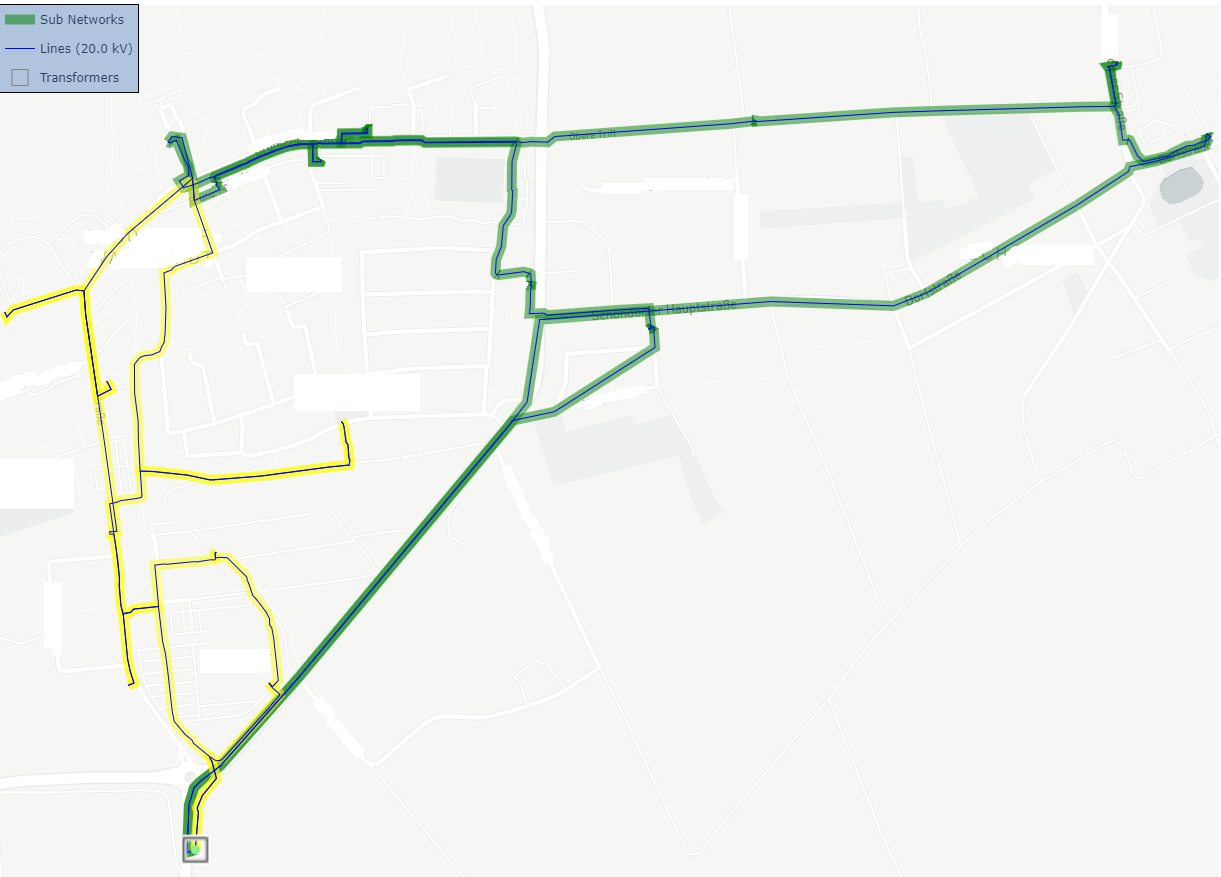
\includegraphics[scale=0.4]{figures/experiments/ringsize/ringsize89_2.png}}
		\caption{Max. 8/9 buses per ring (MV)}
		\label{fig:ringsize89_2}
	\end{centering}
\end{figure}

\begin{figure}[h]
	\begin{centering}
		{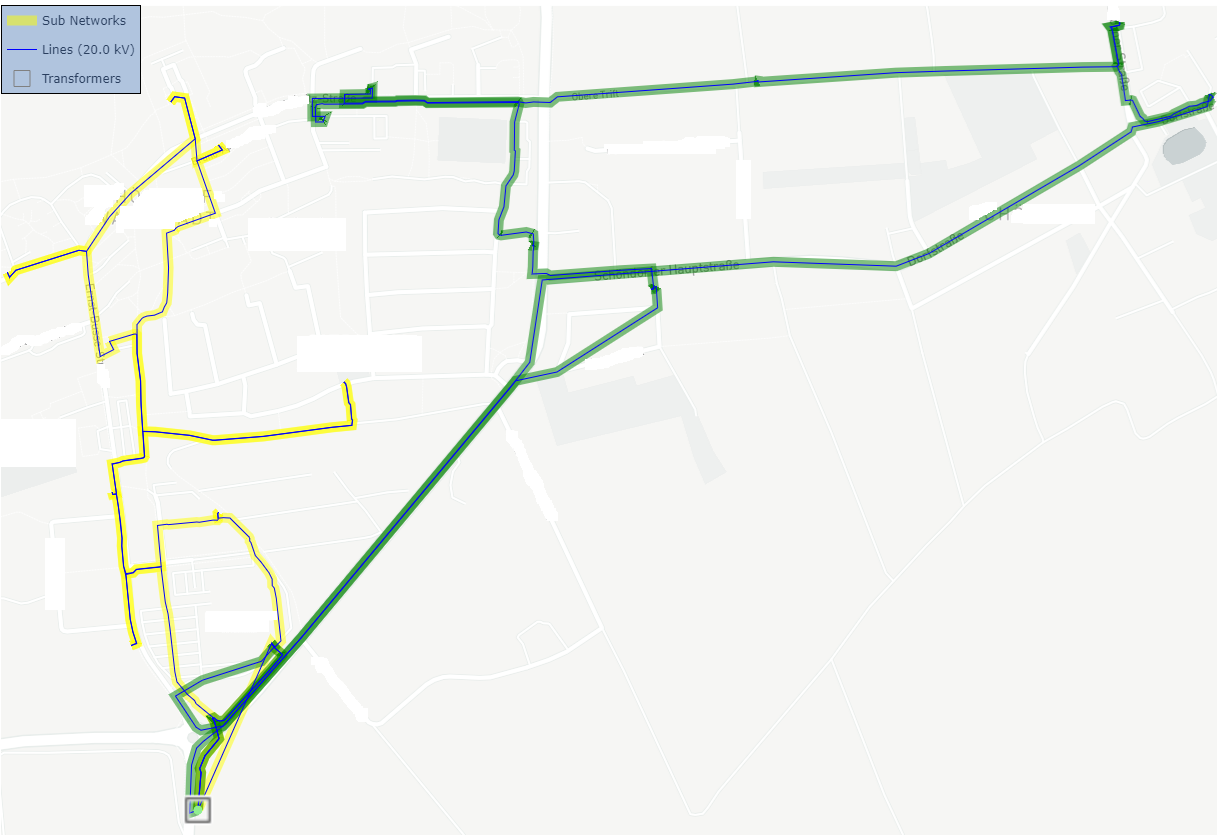
\includegraphics[scale=0.4]{figures/experiments/ringsize/ringsize10_2.png}}
		\caption{Max. ten buses per ring (MV)}
		\label{fig:ringsize10_2}
	\end{centering}
\end{figure}
